\documentclass[a4paper,11pt]{article}	% Classe do documento
%twosides

\title{Geodetic and Surveying Solutions}
\author{Pedro Mendon�a \and Vasco Conde}

%%%%%%%%%%%%%%%%%%%%%%%%%%%%%%%%%%%%%%%

\usepackage [hmargin=3cm,vmargin=3.5cm] {geometry}
%\usepackage[?]{?}

%%%%%%%%%%%%%%%%%%%%%%%%%%%%%%%%%%%%%%%
\usepackage[pdftex]{graphicx}          % suporte para a introdu��o de imagens (ex. jpg e png)
%\usepackage[pdftex,bookmarks=true]{hyperref}

\usepackage{indentfirst}               % espa�o no primeiro paragrafo

\usepackage{fancyhdr}                  % cabe�alho

\usepackage[ansinew]{inputenc}         % suporte a caracteres latinos
\usepackage[T1]{fontenc}               % suporte a hifeniza��o em portugu�s
\usepackage[portuges]{babel}           % suporte a hifeniza��o em portugu�s
\usepackage{ae}                        % Corre��o das fontes por causa do FontEnc/T1

%\usepackage{authordate1-4}            % estilo da bibliografia 

\usepackage[leqno]{amsmath}            % simbolos matematicos
\usepackage{verbatim}                  % verbatim

%mathpackage
\usepackage{ amssymb }

%tabelas
\usepackage{array}
\usepackage{rotating}                  % rodar as tabelas
\usepackage{multirow}                  % jun��o de linhas em tabelas
\usepackage{longtable}                 % tabelas grandes que ocupam mais do que 1 pagina

\usepackage{gensymb}                   % simbolo de graus
\usepackage{eurosym}                   % simbolo de euro

\usepackage{subfig}
\usepackage{float}

\usepackage {enumitem}					% enumerar com 1.1, 1.2, etc
%%%%%%%%%%%%%%%%%%%%%%%%%%%%%%%%%%%%%%%


\begin{document}

%\maketitle

\begin{titlepage}
\begin{center}
%\includegraphics[scale=0.5]{img/logoFCUL.jpg}
\par
%\vspace{1cm}
\textsc{\LARGE Geodetic and Surveying Solutions}
\par
\vspace{7cm}
\centering \LARGE \textit{\textbf{Polly}} 
\par
\vspace{2cm}
\centering \normalsize Traverse Computation
\par
\vspace{9cm}
\centering \textbf{\large Pedro Mendon�a e Vasco Conde}
\par
\large \verb+{plsm.mail, vasconde}@gmail.com+
\par
\vspace{1cm}
%\centering \large Lisboa
\par
\centering \large Lisboa, 2012
\end{center}
\end{titlepage}                    % capa

\pagestyle{fancy}
%\renewcommand{\sectionmark}[1]%
%{\markboth{\MakeUppercase{\thesection.\ #1}}{}}
%\renewcommand{\sectionmark}[1]%
%{\markright{\MakeUppercase{\thesection.\ #1}}}
\renewcommand{\headrulewidth}{0.5pt}
\renewcommand{\footrulewidth}{0.5pt}
\newcommand{\helv}{%
\fontfamily{phv}\fontseries{b}\fontsize{9}{11}\selectfont}
\fancyhf{}
%\fancyhead[LE,RO]{\helv \thepage}
%\fancyfoot[LE,RO]{\helv \thepage}
\fancyfoot[L]{\helv FCUL 2011}
\fancyfoot[R]{\helv \thepage}
\fancyhead[C]{\helv Polly - Traverse Computation}
%\fancyhead[L]{\helv \leftmark}
\fancypagestyle{plain}{%
\fancyhead{} % get rid of headers
\renewcommand{\headrulewidth}{0pt} % and the line
}

\makeatletter
\def\cleardoublepage{\clearpage\if@twoside \ifodd\c@page\else
\hbox{}
\vspace*{\fill}
\begin{center}

\end{center}
\vspace{\fill}
\thispagestyle{empty}
\newpage
\if@twocolumn\hbox{}\newpage\fi\fi\fi}
\makeatother

%\fontfamily{phv}\fontseries{b}\fontsize{9}{11}\selectfont}            % cabe�alho

\newpage

\tableofcontents

\newpage

\section{Observ�veis}

Numa poligonal existir�o esta��es fixas, v�rtices de coordenadas conhecidas, e esta�oes n�o fixas, v�rtices de coordenadas que se pretende determinar. Atrav�s do estacionamento nos diversos v�rtices da poligonal retirar-se-�o observa��es visando a esta��o atr�s e � frente tanto na directa como na inversa, obtendo-se assim 4 visadas em cada estacionamento. As observ�veis s�o as seguintes:

	\underline{Esta��o}:
	\begin{itemize}
	\item ID
	\item Altura Esta��o
	\end{itemize}

	\underline{Vizadas}:
	\begin{itemize}
	\item ID
	\item Medi��o Angular
	\item Dist�ncia Inclinada
	\item Altura Alvo
	\end{itemize}

	\begin{figure}[!htbp] 
    	\centering
    	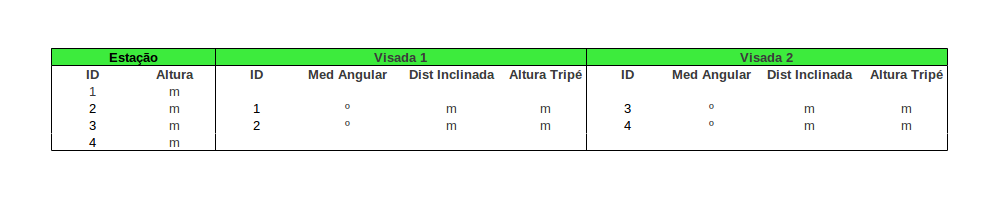
\includegraphics[scale=0.5]{img/Observaveis.png}
    	\caption{Tabela de observ�veis de input.}
    	\label{fig:tabelaObservaveis}
	\end{figure}	

	\newpage

\section{Modelos Matematicos}
	
	Coordenadas:
	\begin{equation*}
	E_j = \sin (R_{ij}) * DH_{ij} + E_i + \epsilon
	\end{equation*}	
	
	\begin{equation*}
	N_j = \cos (R_{ij}) * DH_{ij} + N_i + \epsilon
	\end{equation*}	

	\begin{equation*}
	Z_j = \cos (\measuredangle z_{ij}) * DI_{ij} + Z_i - (h_j - h_i) + \epsilon
	\end{equation*}	
	
	Rumos:
	\begin{equation*}
	R_{ij} = R_{0} + \measuredangle _j + \epsilon (R_0)
	\end{equation*}		

	\begin{equation*}
	R_{0} = R_{-1} + 180 \degree - \measuredangle _{i-1} + \epsilon (R_0)
	\end{equation*}		
	
	
	\newpage
	
\section{Procedimento}

\newpage

\section{Exemplo}

\newpage

\section{Bibliografia}




\end{document}